\documentclass{standalone}
\usepackage{tikz}
\begin{document}
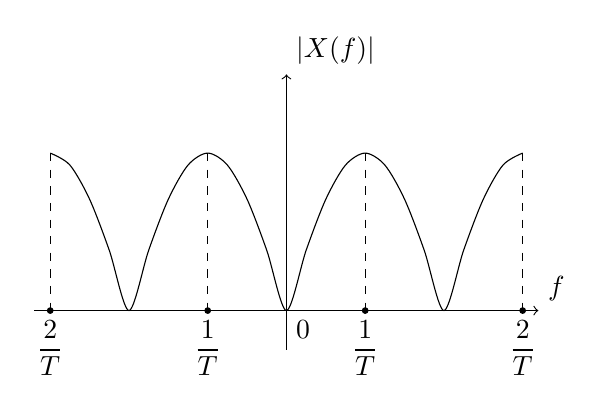
\begin{tikzpicture}[scale=2]
    \draw[->](-1.6,0)--(1.6,0)node[above right]{$f$};
    \draw[->](0,-0.25)--(0,1.5)node[above right]{$|X(f)|$};
    \node[below right]at(0,0){$0$};

    \draw[-]plot[smooth, domain=-1.5:1.5](\x,{abs(sin(pi*\x r))});
    \draw[dashed](0.5,1)--(0.5,0)node[below]{$\displaystyle\frac{1}{T}$};
    \draw[dashed](-0.5,1)--(-0.5,0)node[below]{$\displaystyle\frac{1}{T}$};
    \draw[dashed](1.5,1)--(1.5,0)node[below]{$\displaystyle\frac{2}{T}$};
    \draw[dashed](-1.5,1)--(-1.5,0)node[below]{$\displaystyle\frac{2}{T}$};
    \filldraw[black](0.5,0)circle(0.5pt);
    \filldraw[black](-0.5,0)circle(0.5pt);
    \filldraw[black](1.5,0)circle(0.5pt);
    \filldraw[black](-1.5,0)circle(0.5pt);
\end{tikzpicture}
\end{document}